%%%% Paramétrage du cours %%%%
\def\xxactivite{Cours}

\def\xxauteur{Xavier Pessoles}
\fichefalse \proftrue \tdfalse \courstrue

\def\xxnumchapitre{Chapitre 6 \vspace{.2cm}}
\def\xxchapitre{\hspace{.12cm} Méthode de programmation}

\def\xxcompetences{%
\textsl{%
\textbf{Savoirs et compétences :}\\
\begin{itemize}[label=\ding{112},font=\color{bleuxp}] 
\item Spécifications des données attentdues en entrée et fournie en sortie/retour.
\item Annotation d'un bloc d'instructions par une précondition, une postcondition, une propriété invariante
\item Assertion.
\item Jeu de tests associé à un programme.
\end{itemize}
}}

\def\xxfigures{
%
\includegraphics[width=\linewidth]{fractale}
%\\
%\textit{Modèle du pilote hydraulique avec pilotage interactif.}
}%figues de la page de garde

\input{\repRel/Style/pagegarde_cours_minitoc}
\setlength{\columnseprule}{.1pt}

\vspace{2cm}
\pagestyle{fancy}
\thispagestyle{plain}

%%%%%%%%%%%%%%%%%%%%%%%



\section{Contexte}
Soit la fonction suivante : 
\begin{lstlisting}
def fonction(x,y = []) :
    if x == [] : 
        return y
    else : 
        z = x.pop(0)
        if z not in y : 
            y.append(z)
        return fonction(x, y)
\end{lstlisting}

\textbf{Problèmes :}
\begin{itemize}
\item à quoi sert cette fonction ?
\item quels sont les paramètres à donner ? leur type ?
\item que renvoie la fonction ?
\end{itemize}

Lors de l'écriture d'une fonction, on peut être amener à l'utiliser, le jour même, le lendemain, une semaine plus tard, un mois plus tard... On peut être amener à la partager lorsqu'on travaille sur un projet. 
Il est donc essentiel de les documenter, de les commenter.

Présentons donc les choses ainsi. 

\begin{lstlisting}
def supprimer_doublons_liste(L,y = []) :
    """
    Fonction permettant de renvoyer, à partir d'une liste d'entiers, une liste privée des doublons. 
    La liste initiale sera vidée. 
    """
    if L == [] : 
        return y
    else : 
        z = L.pop(0)
        if z not in y : 
            y.append(z)
        return fonction(L, y)
\end{lstlisting}

En modifiant le nom de la fonction et en ajoutant une court commentaire, il devient plus simple de partager la fonction ou de la réutiliser plus tard. 

\textbf{Problèmes (encore des problèmes) :}
\begin{itemize}
\item on veut une fonction qui supprime les doublons d'une liste d'entiers... comment est-on sûrs que la fonction atteint bien cet objectif ?
\end{itemize}
 
Pour prouver qu'un algorithme on peut envisager deux méthodes : 
\begin{itemize}
\item une méthode empirique (expérimentale) se basant sur des tests, sur le contrôle, des données d'entrées. Cette méthode à l'avantage d'être relativement simple à mettre en \oe{}uvre. Elle a l'inconvénient de valider le comportement d'une fonction sur des cas << ponctuels >>. On ne montre donc pas qu'elle fonctionne dans le cas général. 
\item une méthode formelle, dans le cadre de laquelle on va prouver mathématiquement qu'une fonction atteint bien l'objectif fixé. On parle alors de de terminaison et de correction de l'algorithme.
\end{itemize}

La première méthode fait l'objet du présent chapitre. La seconde fera l'objet d'un chapitre ultérieur. 




\section{Spécification d'une fonction}

\subsection{Spécification à l'aide de commentaires}
\begin{defi}{Signature}
La \textbf{signature d'une fonction} définit les entrées et les sorties d'une fonction. 
\end{defi}

La signature peut comporter par exemple le type  des paramètres d'entrées ou de sorties, des conditions sur ces paramètres. 

La façon la plus simple de signer une fonction, est d'indiquer des commentaires juste après la déclaration de la fonction. 

\begin{exemple}~\\
\begin{lstlisting}
def supprimer_doublons_liste(L,y = []) :
    """
    Fonction permettant de supprimer les doublons d'une liste.
    Entrée : 
     * L: list(int) : liste d'entiers. 
    Sortie : 
     * list(int) : liste d'entiers ne comportant aucun doublons.
    """
    if L == [] : 
        return y
    else : 
        z = L.pop(0)
        if z not in y : 
            y.append(z)
        return fonction(L, y)
\end{lstlisting}

Lorsque les commentaires d'une fonction sont déclarés ainsi après la déclaration d'une fonction (triples \texttt{"}), \texttt{Python} génère automatiquement une documentation en utilisant l'instruction \texttt{help(supprimer\_doublons\_liste)}. On parle de \texttt{docstring}.
\end{exemple}


\subsection{Annotation d'une fonction-- Limite du programme}

Depuis la version 3.5 de \texttt{Python} il est possible d'annoter les fonctions. 
\begin{defi}{} Les annotations de type permettent de donner une information sur le type attendu d'une fonction. Ce ne sont que des indications pour le programmeur. Rien ne l'empêche de ne pas les respecter. 
\end{defi}

\begin{exemple}~\\
%\vspace{-.5cm}
\begin{minipage}[c]{.45\linewidth}
\begin{lstlisting}
def addition(a:int, b:int) -> int : 
    return a+b
\end{lstlisting}
\end{minipage} \hfill
\begin{minipage}[c]{.45\linewidth}
\begin{lstlisting}
>>> addition(1,1)
        2
>>> addition('a','a')
        aa
\end{lstlisting}
\end{minipage} 

\end{exemple}

Comme précisé, les annotations ne sont que des indications. Mais il pourrait être intéressant de pouvoir s'assurer que l'utilisateur de la fonction respecte les conditions d'utilisation de la fonction que ce soit le type des arguments, ou d'autres conditions.

\begin{rem}
En Python, il est possible d'utiliser \texttt{mypy} qui permet de vérifier que lors de l'appel d'une fonction, le typage précisé dans les annotations est bien respecté. 
\end{rem}



\section{Assertion}
\subsection{Validation des entrées}
Comme suite au paragraphe précédent, en phase de debuggage (ou développement), par opposition à la phase de production, \texttt{Python} prévoit la possibilité de vérifier que les arguments donnés à une fonction respectent bien les préconisations du concepteur. 

En utilisant l’instruction \texttt{assert}, le programme s'interrompt quand une erreur est détectée. 

\begin{exemple}
Dans la lignée des annotations de type, on peut tester le type d'argument donné à une fonction. 
\begin{minipage}[c]{.45\linewidth}
\begin{lstlisting}
def addition(a:int, b:int) -> int : 
    assert type(a) == int and type(b) == int
    return a+b
\end{lstlisting}
\end{minipage} \hfill
\begin{minipage}[c]{.45\linewidth}
\begin{lstlisting}
>>> addition(1,1)
        2
>>> addition('a','a')
        (...)
        AssertionError
\end{lstlisting}
\end{minipage} 

Si les arguments sont du mauvais type, \texttt{Python} déclenche une \texttt{AssertionError}.
\end{exemple}


\begin{exemple} Prenons un type d'exemple que nous rencontrerons plus souvent : l'algorithme fonctionne seulement si des préconditions sont remplies. 

Par exemple dans le cas de la résolution de l'équation $f(x)=0$, il est nécessaire que $f$ soit continue, monotone et que $f(a)$ et $f(b)$ soient de signes différents. Il faut aussi que $\varepsilon$ soit positif. On peut donc procéder de la façon suivante. 

\begin{lstlisting}
def dichotomie(f, a:float , b:float , epsilon:float) -> float :
    """Zéro de f sur [a,b] à epsilon près, par dichotomie
        Préconditions : f(a) * f(b) <= 0
        f continue sur [a,b]
        epsilon > 0"""
    assert (f(a) * f(b) <= 0) and (epsilon > 0)
    c, d = a, b
    fc, fd = f(c), f(d)
    while d - c > 2 * epsilon:
        m = (c + d) / 2.
        fm = f(m)
        if fc * fm <= 0:
            d, fd = m, fm
        else:
            c, fc = m, fm
    return (c + d) / 2.
\end{lstlisting}
\end{exemple}

\subsection{Vers la gestion d'exceptions -- hors programme}
L'avantage des assertions et leur facilité à être mise en \oe{}uvre. L'inconvénient et qu'il n'est pas possible de savoir précisément ce qui a généré l'erreur d'assertion : un problème de précondition ? de type ? autre ?

Du fait de leur manque de précision, il peut être difficile de les gérer. 

Un premier pas vers la gestion d'erreur est de donner à l'utilisateur la raison pour laquelle la fonction génère une erreur. 
Pour cela, on va \textit{lever une exception}.

\begin{lstlisting}
def dichotomie(f, a:float , b:float , epsilon:float) -> float :
    """Zéro de f sur [a,b] à epsilon près, par dichotomie
        Préconditions : f(a) * f(b) <= 0
        f continue sur [a,b]
        epsilon > 0"""
    if f(a) * f(b) > 0 : 
        raise Exception("f(a) et f(b) sont de même signe")
    elif epsilon < 0 :
        raise Exception("epsilon est négatif")

    c, d = a, b
    fc, fd = f(c), f(d)
    while d - c > 2 * epsilon:
        m = (c + d) / 2.
        fm = f(m)
        if fc * fm <= 0:
            d, fd = m, fm
        else:
            c, fc = m, fm
    return (c + d) / 2.
\end{lstlisting}

\begin{lstlisting}
>>> dichotomie(f, 0, 1, 0.00001)
   (...)
   Exception: f(a) et f(b) sont de même signe
\end{lstlisting}

\section{Génération de tests}

\subsection{Tests unitaires}

On a vu comment vérifier que les données d'entrées d'une fonction sont compatibles avec ce qu'attendait le concepteur de la fonction. On va maintenant chercher, grâce à des tests unitaires, si le résultat attendu est bien celui déterminé par une fonction. 
\begin{exemple}~\\
\begin{minipage}[c]{.5\linewidth}
\begin{lstlisting}
def addition(a:int, b:int) -> int : 
    assert type(a) == int and type(b) == int
    return a+b
\end{lstlisting}
\end{minipage} \hfill
\begin{minipage}[c]{.45\linewidth}
\begin{lstlisting}
>>> addition(1,1) == 2
        True
>>> addition(1,1) == 3
        False
\end{lstlisting}
\end{minipage} 

\end{exemple}

Ces tests ont l'avantage d'être simples à mettre en \oe{}uvre mais ne garantissent pas que la fonction << marche >> dans tous les cas. 

Il est alors possible de créer une fonction de tests. 
\begin{lstlisting}
def test_addition() :
    assert addition(1,1) == 2
    assert addition(1,1) !=3
\end{lstlisting}

Des jeux de tests pertinents peuvent être des tests sur les cas limites. 
Dans le cas de la recherche dichotomique, on peut se demander si la boucle \texttt{while} n'est pas réalisée une fois de trop par rapport à la valeur de \texttt{epsilon}.

\begin{lstlisting}
>>> res = dichotomie(f, 0, 1, epsilon)
>>> f(res) < epsilon # MAUVAIS test : f(res) peut être négatif
    True
>>> abs(f(res)) < epsilon 
    False 
>>> # L'algorithme dichotomique doit itérer une fois de plus ?
\end{lstlisting}

En modifiant l'algorithme, et en itérant une fois de plus, le test reste faux. La condition d'arrêt de l'algorithme ne permet pas de trouver x tel que $f(x)<\varepsilon$ mais de trouver une valeur de $x$ telle que l'écart entre deux solutions consécutives est inférieur à $\varepsilon$. Il faut donc clarifier l'objectif de la fonction pour proposer un test plus adapté.



\subsection{Vers Pytest -- hors programme}

Lorsqu'on connaît dans un grand nombre de cas le résultat qui est sensé être trouvé par une fonction, il est possible de faire passer une batterie de tests à cette fonction en recherchant si le résultat calculé et bien le résultat attendu. 

Soit la fonction suivante permettant de calculer le produit scalaire entre deux vecteurs. 
\begin{lstlisting}
def produit_scalaire_v2(vecteur1, vecteur2):
    somme = 0
    for i in range(len(vecteur1)):
        somme += vecteur1[i]*vecteur2[i]+1
    return somme
\end{lstlisting}

\texttt{Pytest} permet de faire passer une batterie de tests à une fonction. Ces tests sont des fonctions commençant obligatoirement par \texttt{test\_}.

\begin{lstlisting}
def test_produit_scalaire_v2_01():
    assert produit_scalaire_v2([1, 1, 1], [1, 1, 1]) == 3

def test_produit_scalaire_v2_02():
    assert produit_scalaire_v2([1, 2, 3, 4], [0, 1, 0, 0]) == 2
\end{lstlisting}

Le lancement de \texttt{Pytest} donne le résultat suivant. 

\begin{center}
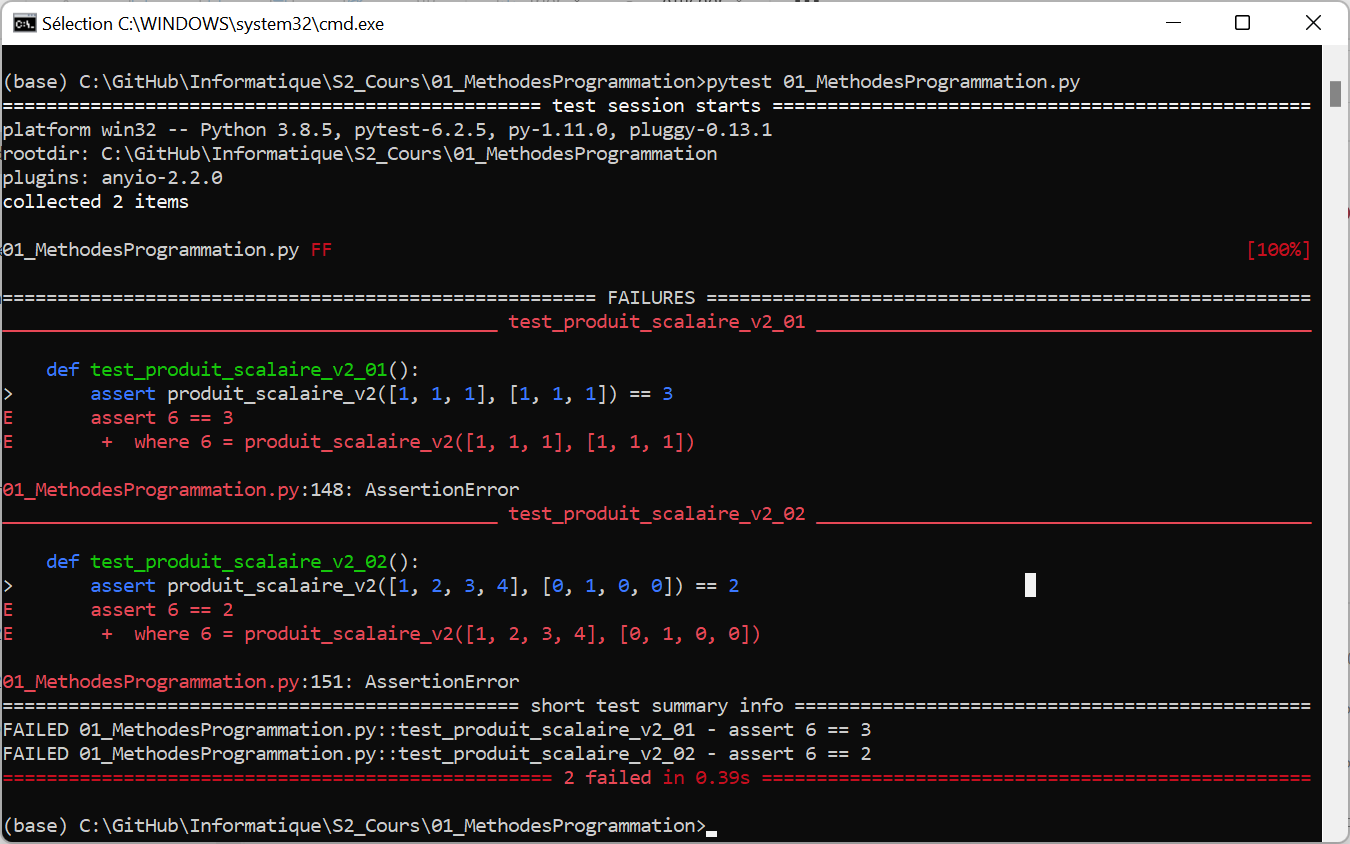
\includegraphics[width=.8\linewidth]{pytest}
\end{center}


On peut lire que les deux tests ont échoué. La fonction ne remplit donc vraisemblablement pas son objectif. 

% https://mypy.readthedocs.io/en/stable/cheat_sheet_py3.html
